
\documentclass[11pt]{amsbook}

\usepackage{../HBSuerDemir}
\usepackage{wrapfig}
\graphicspath{ {images/} }

\begin{document}
    % ++++++++++++++++++++++++++++++++++++++
    \hPage{b2p1/126}
    % ++++++++++++++++++++++++++++++++++++++
    
    Generalizing, we have 
    \[c_1\overrightarrow{P_1} + c_2\overrightarrow{P_2} + ... + c_n\overrightarrow{P_n} = 
\sum_{k=1}^{n} c_k\overrightarrow{P_k} \]
which is called a \underline{linear combination} of n vectors.

\begin{wrapfigure}{r}{40pt}
    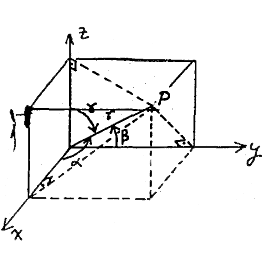
\includegraphics[scale=0.4]{b2p1-126-fig01}
\end{wrapfigure}

\subsubsection{Direction-angles, -cosine and -numbers} : \\
Let $\overrightarrow{r} = \overrightarrow{OP}$ be a positive vector with length r. The angles $\alpha$, $\beta$, $\gamma$ that are made by $\overrightarrow{r}$ with positive sides of axes are \underline{direction angles}, their cosines $\cos\alpha$, $\cos\beta$, $\cos\gamma$ are \underline{direction cosines} and numbers proportional to direction cosines are \underline{direction numbers} of $\overrightarrow{OP}$.

\par Since scalar projections of $P(x, y, z)$ on the axes are x, y, z one has 
\[ \cos\alpha = \frac{x}{r} \text{,} \cos\beta = \frac{y}{r} \text{,} \cos\gamma = \frac{z}{r}\]
and consequently x, y, z and for $k \neq 0$, kx, ky, kz are direction numbers.

\section{Multiplication of Vectors}
There are two kinds of multiplication for vectors. scalar
and vector multiplications, the results of which being scalar and
vector: 
\subsection{Scalar product of two vectors}
Let $A = (a_1, a_2, a_3)$, $B = (b_1, b_2, b_3)$ be two vectors. Then

\[ A.B = |A||B|\cos\theta\]

is called \underline{scalar product} of A and B, where $\theta$ is the angle between them $(0 \leq \theta \leq \pi)$
\end{document}  

